\documentclass{ctexart}
\usepackage{ctex}
\usepackage{geometry}
\usepackage{enumitem}
\usepackage{indentfirst}
\usepackage{color}
\usepackage{fancyhdr}
\usepackage{amsmath}
\usepackage{graphicx}

% 设置纸张和页边距——A4
\geometry{papersize={21cm,29.7cm}}
\geometry{left=3.18cm,right=3.18cm,top=2.54cm,bottom=2.54cm}

% 一级标题靠左
\CTEXsetup[format={\Large\bfseries}]{section}

% 去除页眉
\pagestyle{plain}

% 开始文档内容
\begin{document}

\title{信号与系统课程笔记:Lecture 2}
\author{授课教师:秦雨潇 \\
        笔记记录:李梦薇}
\date{2023 年 09 月 08 日(第一周,周五)}
\maketitle

\section{信号和系统的性质(复习)}
\subsection{信号的性质}
\begin{enumerate}[itemindent=2em,label=(\arabic*)]
    \item 如何识别信息?
    \item 如何处理信号?
\end{enumerate}
\subsection{系统的性质}
\begin{enumerate}[itemindent=2em,label=(\arabic*)]
    \item 如何理解系统?
    \item 如何制造系统?
\end{enumerate}

\section{线性时不变(LTI)系统}
输入信号为 $f(t)$,系统为 $h(t)$,输出信号为 $y(t)$。那么:
% 插入图像
\begin{figure}[htbp]
    \centering
    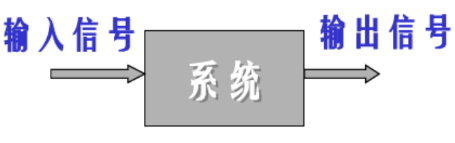
\includegraphics[width=6cm,height=2cm]{系统.png}
    \caption{系统}
\end{figure}
\subsection{时不变性}
若 $f(t)\longrightarrow{y(t)}$,则 $f(t-t_0)\longrightarrow{y(t-t_0)}$
\subsection{线性}
线性是指系统同时具备叠加性和齐次性。\par
若 $f_1(t)\longrightarrow{y_1(t)}$,$f_2(t)\longrightarrow{y_2(t)}$,则 $a_1f_1(t)+a_2f_2(t)\longrightarrow{a_1y_1(t)+a_2y_2(t)}$

\section{学习思路}
\textbf{再次强调}:由简到难,由特殊到一般。

\end{document}